\documentclass[tikz,border=10pt]{standalone}

\usepackage{tikz}
\usetikzlibrary{shapes,arrows,positioning,calc,backgrounds,fit,decorations.pathreplacing}

% MINIX TikZ style guide color palette
\definecolor{primaryblue}{RGB}{41,128,185}
\definecolor{secondarygreen}{RGB}{39,174,96}
\definecolor{accentorange}{RGB}{230,126,34}
\definecolor{warningred}{RGB}{192,57,43}
\definecolor{lightgray}{RGB}{236,240,241}
\definecolor{darkgray}{RGB}{52,73,94}

\begin{document}
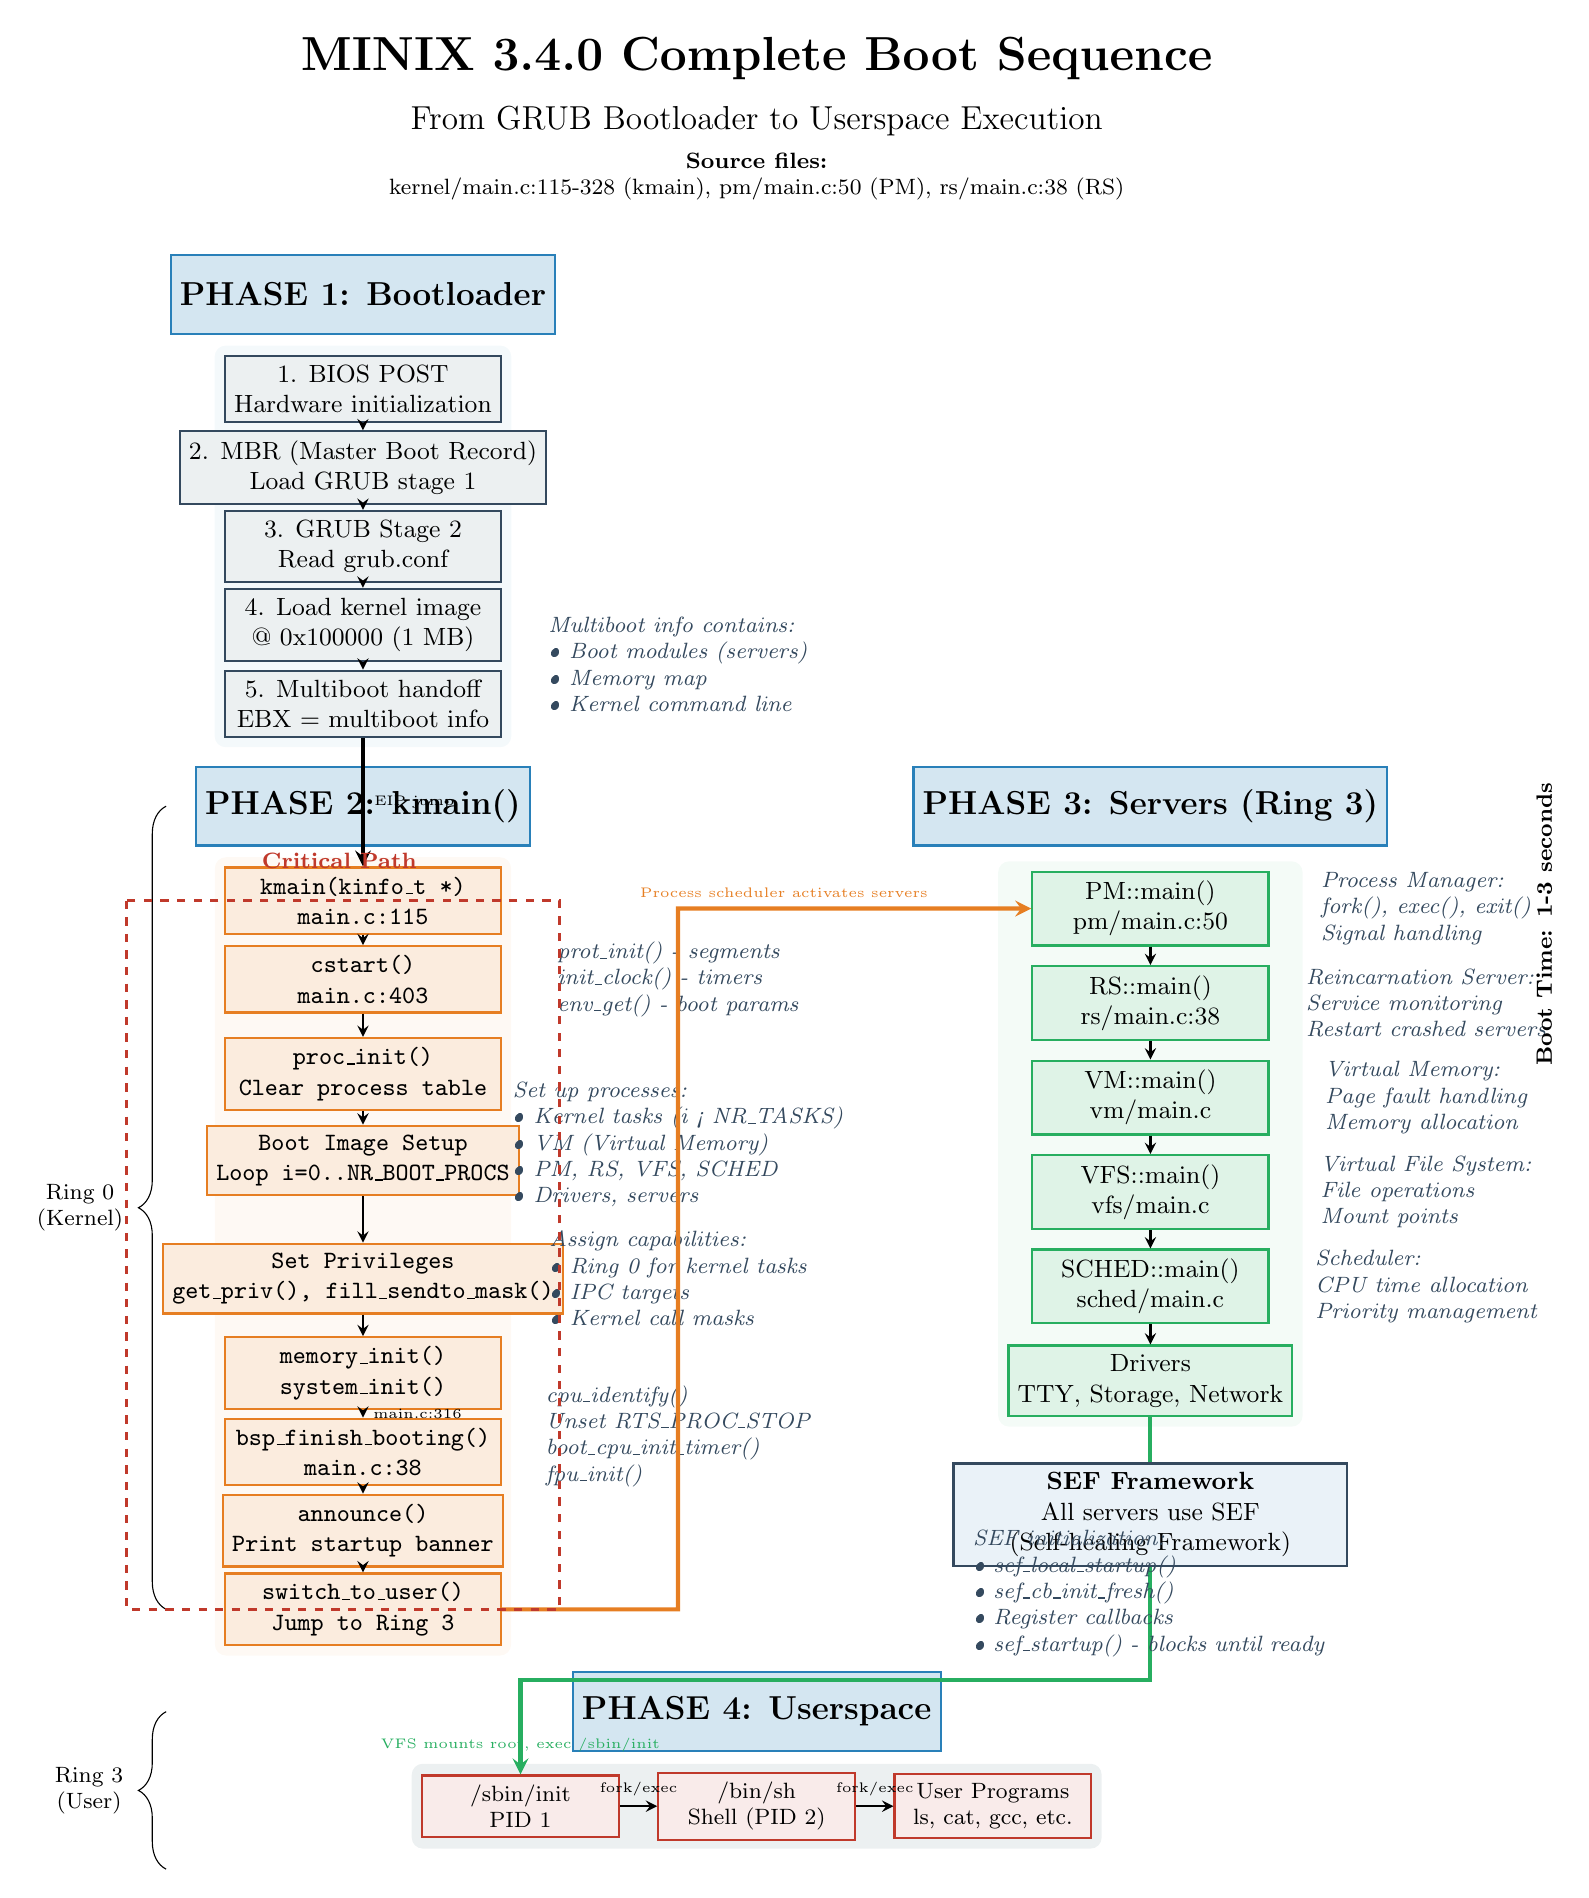
\begin{tikzpicture}[
    % Node styles
    phase/.style={rectangle, draw=primaryblue, fill=primaryblue!20, thick, minimum width=4cm, minimum height=1cm, font=\bfseries\large, align=center},
    box/.style={rectangle, draw=darkgray, fill=lightgray, thick, minimum width=3.5cm, minimum height=0.7cm, font=\small, align=center},
    kernelbox/.style={rectangle, draw=accentorange, fill=accentorange!15, thick, minimum width=3.5cm, minimum height=0.7cm, font=\small\ttfamily, align=center},
    serverbox/.style={rectangle, draw=secondarygreen, fill=secondarygreen!15, thick, minimum width=3cm, minimum height=0.7cm, font=\small, align=center},
    procbox/.style={rectangle, draw=warningred, fill=warningred!10, thick, minimum width=2.5cm, minimum height=0.6cm, font=\footnotesize, align=center},
    arrow/.style={->, >=stealth, thick},
    widearrow/.style={->, >=stealth, very thick, line width=1.5pt},
    dashedarrow/.style={->, >=stealth, thick, dashed},
    label/.style={font=\small, align=center},
    note/.style={font=\footnotesize\itshape, align=left, text=darkgray},
]

% Title
\node[font=\LARGE\bfseries] at (10, 22) {MINIX 3.4.0 Complete Boot Sequence};
\node[font=\large] at (10, 21.2) {From GRUB Bootloader to Userspace Execution};

% Source file reference
\node[font=\footnotesize, align=center] at (10, 20.5) {
    \textbf{Source files:}\\
    kernel/main.c:115-328 (kmain), pm/main.c:50 (PM), rs/main.c:38 (RS)
};

% ============================================================================
% PHASE 1: BOOTLOADER (GRUB)
% ============================================================================

\node[phase] (grub) at (5, 19) {PHASE 1: Bootloader};

\node[box] (bios) at (5, 17.8) {1. BIOS POST\\Hardware initialization};
\node[box] (mbr) at (5, 16.8) {2. MBR (Master Boot Record)\\Load GRUB stage 1};
\node[box] (grub_stage2) at (5, 15.8) {3. GRUB Stage 2\\Read grub.conf};
\node[box] (kernel_load) at (5, 14.8) {4. Load kernel image\\@ 0x100000 (1 MB)};
\node[box] (multiboot) at (5, 13.8) {5. Multiboot handoff\\EBX = multiboot info};

\draw[arrow] (bios) -- (mbr);
\draw[arrow] (mbr) -- (grub_stage2);
\draw[arrow] (grub_stage2) -- (kernel_load);
\draw[arrow] (kernel_load) -- (multiboot);

% Multiboot info structure
\node[note] at (9, 14.3) {
Multiboot info contains:\\
• Boot modules (servers)\\
• Memory map\\
• Kernel command line
};

% ============================================================================
% PHASE 2: KERNEL ENTRY (kmain)
% ============================================================================

\node[phase] (kmain_phase) at (5, 12.5) {PHASE 2: kmain()};

\node[kernelbox] (kmain_entry) at (5, 11.3) {kmain(kinfo\_t *)\\main.c:115};

\draw[widearrow] (multiboot) -- (kmain_entry) node[midway, right, font=\tiny] {EIP jump};

% cstart()
\node[kernelbox] (cstart) at (5, 10.3) {cstart()\\main.c:403};
\node[note] at (9, 10.3) {
prot\_init() - segments\\
init\_clock() - timers\\
env\_get() - boot params
};

\draw[arrow] (kmain_entry) -- (cstart);

% proc_init()
\node[kernelbox] (proc_init) at (5, 9.1) {proc\_init()\\Clear process table};

\draw[arrow] (cstart) -- (proc_init);

% Boot image setup
\node[kernelbox] (boot_image) at (5, 8) {Boot Image Setup\\Loop i=0..NR\_BOOT\_PROCS};
\node[note] at (9, 8.2) {
Set up processes:\\
• Kernel tasks (i < NR\_TASKS)\\
• VM (Virtual Memory)\\
• PM, RS, VFS, SCHED\\
• Drivers, servers
};

\draw[arrow] (proc_init) -- (boot_image);

% Set privileges
\node[kernelbox] (set_priv) at (5, 6.5) {Set Privileges\\get\_priv(), fill\_sendto\_mask()};
\node[note] at (9, 6.5) {
Assign capabilities:\\
• Ring 0 for kernel tasks\\
• IPC targets\\
• Kernel call masks
};

\draw[arrow] (boot_image) -- (set_priv);

% Initialize subsystems
\node[kernelbox] (subsys_init) at (5, 5.3) {memory\_init()\\system\_init()};

\draw[arrow] (set_priv) -- (subsys_init);

% bsp_finish_booting()
\node[kernelbox] (bsp_finish) at (5, 4.3) {bsp\_finish\_booting()\\main.c:38};
\node[note] at (9, 4.5) {
cpu\_identify()\\
Unset RTS\_PROC\_STOP\\
boot\_cpu\_init\_timer()\\
fpu\_init()
};

\draw[arrow] (subsys_init) -- (bsp_finish) node[midway, right, font=\tiny] {main.c:316};

% announce()
\node[kernelbox] (announce) at (5, 3.3) {announce()\\Print startup banner};

\draw[arrow] (bsp_finish) -- (announce);

% switch_to_user()
\node[kernelbox] (switch_user) at (5, 2.3) {\textbf{switch\_to\_user()}\\Jump to Ring 3};

\draw[arrow] (announce) -- (switch_user);

% ============================================================================
% PHASE 3: SERVER INITIALIZATION (Right column)
% ============================================================================

\node[phase] (server_phase) at (15, 12.5) {PHASE 3: Servers (Ring 3)};

% PM Server
\node[serverbox] (pm_main) at (15, 11.2) {PM::main()\\pm/main.c:50};
\node[note] at (18.5, 11.2) {
Process Manager:\\
fork(), exec(), exit()\\
Signal handling
};

% RS Server
\node[serverbox] (rs_main) at (15, 10) {RS::main()\\rs/main.c:38};
\node[note] at (18.5, 10) {
Reincarnation Server:\\
Service monitoring\\
Restart crashed servers
};

% VM Server
\node[serverbox] (vm_main) at (15, 8.8) {VM::main()\\vm/main.c};
\node[note] at (18.5, 8.8) {
Virtual Memory:\\
Page fault handling\\
Memory allocation
};

% VFS Server
\node[serverbox] (vfs_main) at (15, 7.6) {VFS::main()\\vfs/main.c};
\node[note] at (18.5, 7.6) {
Virtual File System:\\
File operations\\
Mount points
};

% SCHED Server
\node[serverbox] (sched_main) at (15, 6.4) {SCHED::main()\\sched/main.c};
\node[note] at (18.5, 6.4) {
Scheduler:\\
CPU time allocation\\
Priority management
};

% Drivers
\node[serverbox] (drivers) at (15, 5.2) {Drivers\\TTY, Storage, Network};

% Transition arrow from kernel to servers
\draw[widearrow, accentorange] (switch_user) -- ++(4,0) -- ++(0,8.9) -- (pm_main)
    node[pos=0.3, above, font=\tiny] {Process scheduler activates servers};

\draw[arrow] (pm_main) -- (rs_main);
\draw[arrow] (rs_main) -- (vm_main);
\draw[arrow] (vm_main) -- (vfs_main);
\draw[arrow] (vfs_main) -- (sched_main);
\draw[arrow] (sched_main) -- (drivers);

% ============================================================================
% PHASE 4: USERSPACE PROCESSES (Bottom)
% ============================================================================

\node[phase] (userspace_phase) at (10, 1) {PHASE 4: Userspace};

% Init process
\node[procbox] (init_proc) at (7, -0.2) {/sbin/init\\PID 1};

% Shell
\node[procbox] (shell) at (10, -0.2) {/bin/sh\\Shell (PID 2)};

% User programs
\node[procbox] (user_prog) at (13, -0.2) {User Programs\\ls, cat, gcc, etc.};

\draw[widearrow, secondarygreen] (drivers) -- ++(0,-3.8) -- ++(-8,0) -- (init_proc)
    node[pos=0.5, below, font=\tiny] {VFS mounts root, exec /sbin/init};

\draw[arrow] (init_proc) -- (shell) node[midway, above, font=\tiny] {fork/exec};
\draw[arrow] (shell) -- (user_prog) node[midway, above, font=\tiny] {fork/exec};

% SEF Framework note
\node[box, fill=primaryblue!10, minimum width=5cm] at (15, 3.5) {
\textbf{SEF Framework}\\
All servers use SEF\\
(Self-healing Framework)
};

\node[note, text width=4.5cm] at (15, 2.5) {
SEF initialization:\\
• sef\_local\_startup()\\
• sef\_cb\_init\_fresh()\\
• Register callbacks\\
• sef\_startup() - blocks until ready
};

% ============================================================================
% EXECUTION FLOW ANNOTATIONS
% ============================================================================

% Ring transition annotation
\draw[decorate, decoration={brace, amplitude=10pt, mirror}]
    (2.5, 12.5) -- (2.5, 2.3) node[midway, left=12pt, align=center, font=\footnotesize] {Ring 0\\(Kernel)};

\draw[decorate, decoration={brace, amplitude=10pt, mirror}]
    (2.5, 1) -- (2.5, -1) node[midway, left=12pt, align=center, font=\footnotesize] {Ring 3\\(User)};

% Timeline annotation (right side)
\node[font=\footnotesize\bfseries, rotate=90] at (20, 11) {Boot Time: 1-3 seconds};

% Critical path marker
\draw[warningred, very thick, dashed]
    (2, 11.3) rectangle (7.5, 2.3);
\node[font=\footnotesize\bfseries, text=warningred] at (4.7, 11.8) {Critical Path};

% Background zones
\begin{pgfonlayer}{background}
    % Bootloader zone
    \node[fill=primaryblue!5, rounded corners, fit=(bios) (multiboot)] {};

    % Kernel zone
    \node[fill=accentorange!5, rounded corners, fit=(kmain_entry) (switch_user)] {};

    % Server zone
    \node[fill=secondarygreen!5, rounded corners, fit=(pm_main) (drivers)] {};

    % Userspace zone
    \node[fill=lightgray, rounded corners, fit=(init_proc) (user_prog)] {};
\end{pgfonlayer}

\end{tikzpicture}
\end{document}
